\section{Uncertainty Variation in Data Distribution Shapes the River Valley Landscape}
\label{sec:data}

What causes the loss landscape to resemble a river valley structure? In this section, we propose and validate the hypothesis that variations in next-token uncertainty shape the loss landscape. When predicting a deterministic fact, a large learning rate can boost the model's confidence, accelerating learning. However, when the next token is inherently ambiguous—such as the continuation of a phrase like "I am"—the model must learn a calibrated distribution, which may necessitate a smaller step size. This variation in uncertainty leads to differences in sharpness across the loss landscape, resulting in the river valley structure.


\textbf{A Toy Bigram Language.} We formalize this intuition using a synthetic language composed of cities and names, where each city corresponds to a unique distribution of its citizens' names. For instance, one city might have a highly deterministic distribution, with most residents named "Ken``, while another city may have a more diverse {distribution of names}. This synthetic language follows the structure in~\cite{allenzhu2024physicslanguagemodels33}. The goal is to learn the distribution of names conditioned on each city. We show that cities with more deterministic name distributions align with flatter regions in the loss landscape (the "river"). In contrast, cities with more diverse name distributions correspond to sharper regions (the "hillsides").

\begin{wrapfigure}{r}{0.34\textwidth}
    \centering
    \vspace{-0.3in}
    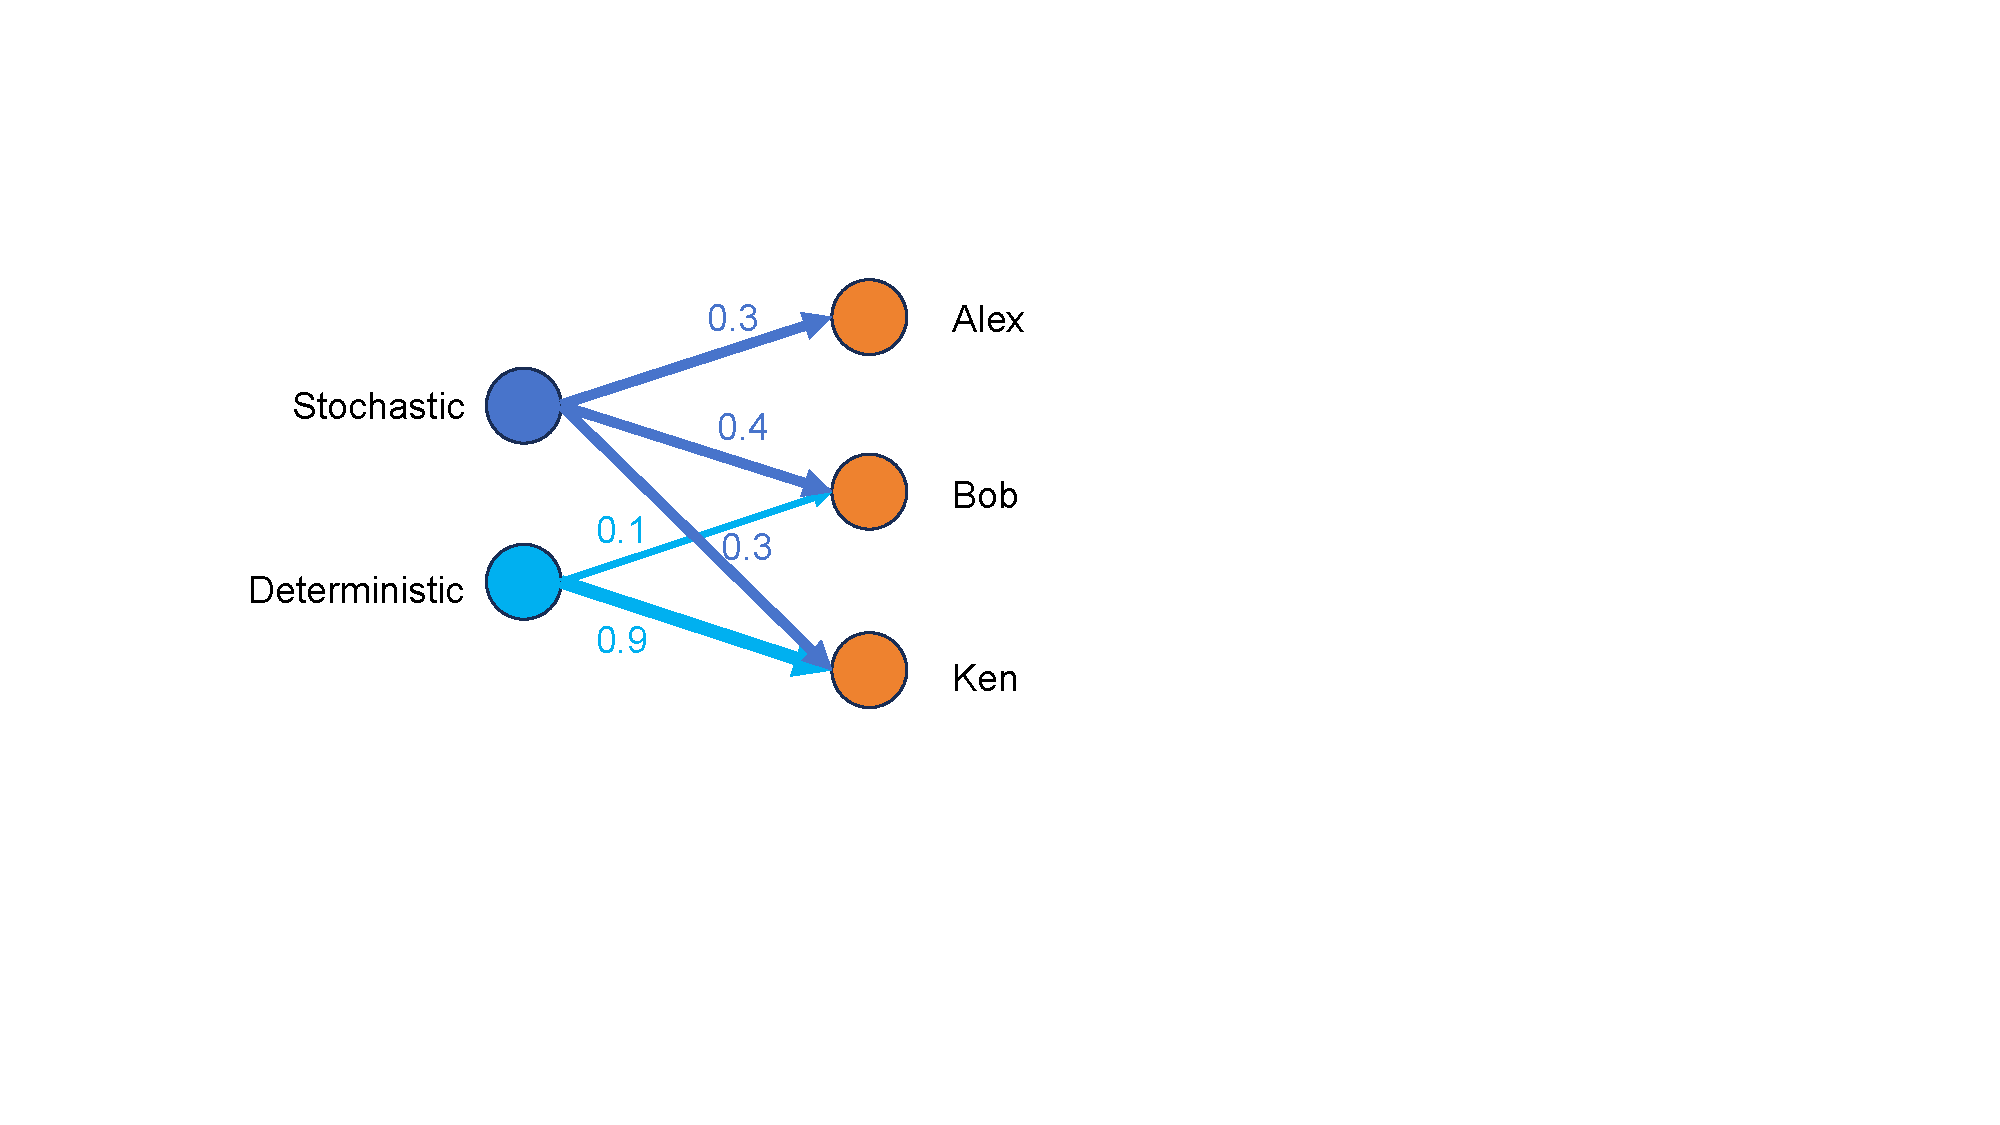
\includegraphics[width=0.3\textwidth]{figures/arxiv/city.pdf}
    \caption{\textbf{Visualization of Toy Bigram Language.} We design a synthetic dataset where each city has a unique name distribution. The left shows the name distributions for two cities, one deterministic and one stochastic.}
    \label{fig:data}
    \vspace{-0.4in}
\end{wrapfigure}

Formally, let the set of cities be represented by \(\{1, \ldots, n\}\) and the set of names by \(\{1, \ldots, m\}\). Data is generated by first selecting a city \(i\) uniformly at random, then sampling a name \(j\) according to the city's name distribution. The \emph{name distribution} for city \(i\) is parameterized by a categorical distribution \(\mathrm{Categorical}([P_{i,j}]_{j=1}^m)\), where \(P_{i,j}\) represents the probability of selecting name \(j\) in city \(i\), and each \(P_{i,j} > 0\).
To quantify the uncertainty in each city’s name distribution, we compute the Gini impurity of the distribution as:
\[
U_i = \mathrm{I_G}(\mathrm{name} \mid \mathrm{city} = i) = 1 - \sum_{j = 1}^m P_{i,j}^2 \in \left[0, 1 - \frac{1}{m} \right).
\]

The value of $U_i$ reflects the uncertainty of city $i$'s name distribution. When the distribution is close to deterministic—i.e., there exists a $j$ such that $P_{i,j}$ is near 1—$U_i$ approaches its lower bound of 0. Conversely, for a nearly uniform distribution, $U_i$ approaches its upper bound of $1 - \frac{1}{m}$. 
Given this setup, we parameterize our model with $\Theta \in \mathbb{R}^{n \times m}$, where each row corresponds to a city and each column to a name. The model estimates the probability of name $j$ for city $i$ using the softmax function $\frac{\exp(\Theta_{i,j})}{\sum_{k=1}^m \exp(\Theta_{i,k})}$.

We use sampled data to train this model. Specifically, for each sampled city $i$, a name $j$ is drawn according to the true distribution $\mathcal{P}_{i,j}$. The model's task is to predict the correct name based on the sampled city, minimizing the negative log-likelihood (NLL) over the sampled data. 
The population loss is given by:
\begin{align}
\label{eq:toy}
    L(\Theta) = \frac{1}{n} \sum_{i = 1}^n \ell_i(\Theta_{i,:}) ,\quad
\ell_i(\Theta_{i,:}) = -\sum_{j = 1}^m \mathcal{P}_{i,j} \log \frac{\exp(\Theta_{i,j})}{\sum_{k=1}^m \exp(\Theta_{i, k})}.
\end{align}


This loss is separable across different cities, meaning that the contribution from each city is independent. The loss component $\ell_i(\Theta_{i,:})$ captures the contribution from city $i$, and different name distributions across cities lead to different forms of $\ell_i$.
Considering a parameter $\Theta^*$ that minimizes the loss $L$, we will show that cities with more stochastic name distributions correspond to sharper components in the loss landscape, as reflected by the average-direction sharpness of $\ell_i$ ($\mathrm{Tr}(\nabla^2 \ell_i(\theta)) \mid_{\theta = \Theta^*_{i,:}}$). 


\begin{lemma}
\label{lem:sharp}
The average-direction sharpness of loss component $\ell_i$ at $\Theta^*$ equals the uncertainty of the name distribution ($U_i$).
$\mathrm{Tr}(\nabla^2 \ell_i(\theta)) \mid_{\theta = \Theta^*_{i,:}} = U_i.$
\end{lemma}
\Cref{lem:sharp} demonstrates that at the global minimum, the sharpness associated with a city decreases as the city's name distribution becomes more deterministic. This aligns with the intuition that a deterministic token corresponds to a flatter loss direction.

In a generalized river valley landscape, the hillsides represent the sharper components of the loss, which in this context correspond to cities with more stochastic name distributions. Conversely, the river corresponds to cities with more deterministic name distributions. We can further establish the existence of a generalized river (\Cref{assum:gen-river}) in this loss landscape under appropriate assumptions about $\mathcal{P}$ (see \Cref{thm:toy}). Along the river, the gradient remains nonzero only for the cities with more deterministic name distributions, reinforcing the connection between determinism and flatness in the loss landscape.


\begin{figure}[!h]
    \centering
    \begin{subfigure}[b]{0.45\textwidth}
        \centering
        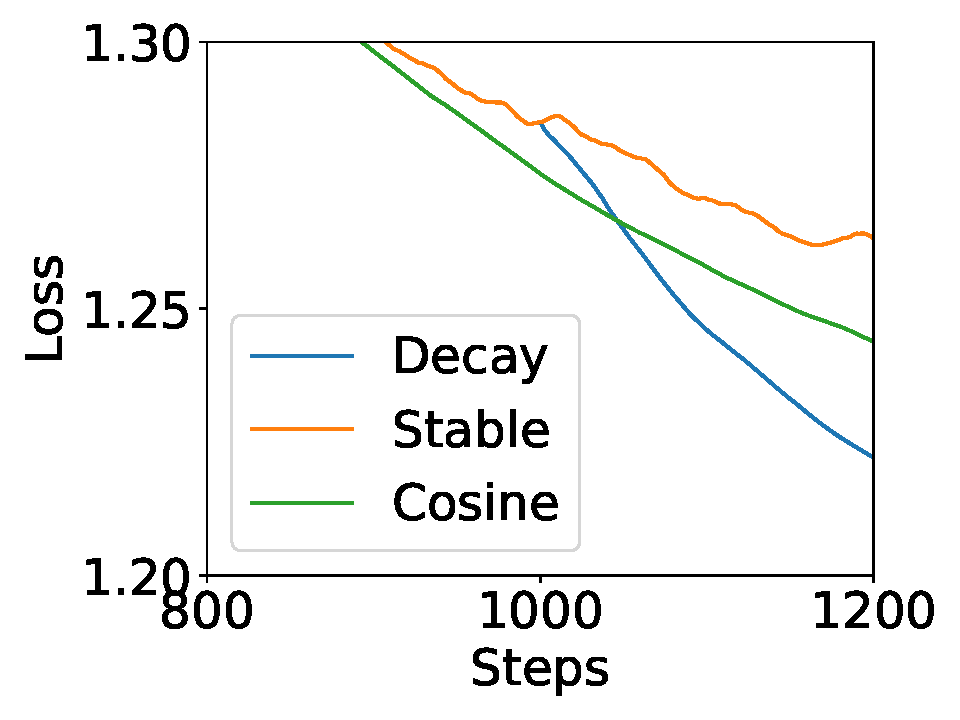
\includegraphics[width=\textwidth]{figures/arxiv/toy_pit.pdf}
    \end{subfigure}
    \hfill
    \begin{subfigure}[b]{0.54\textwidth}
        \centering
        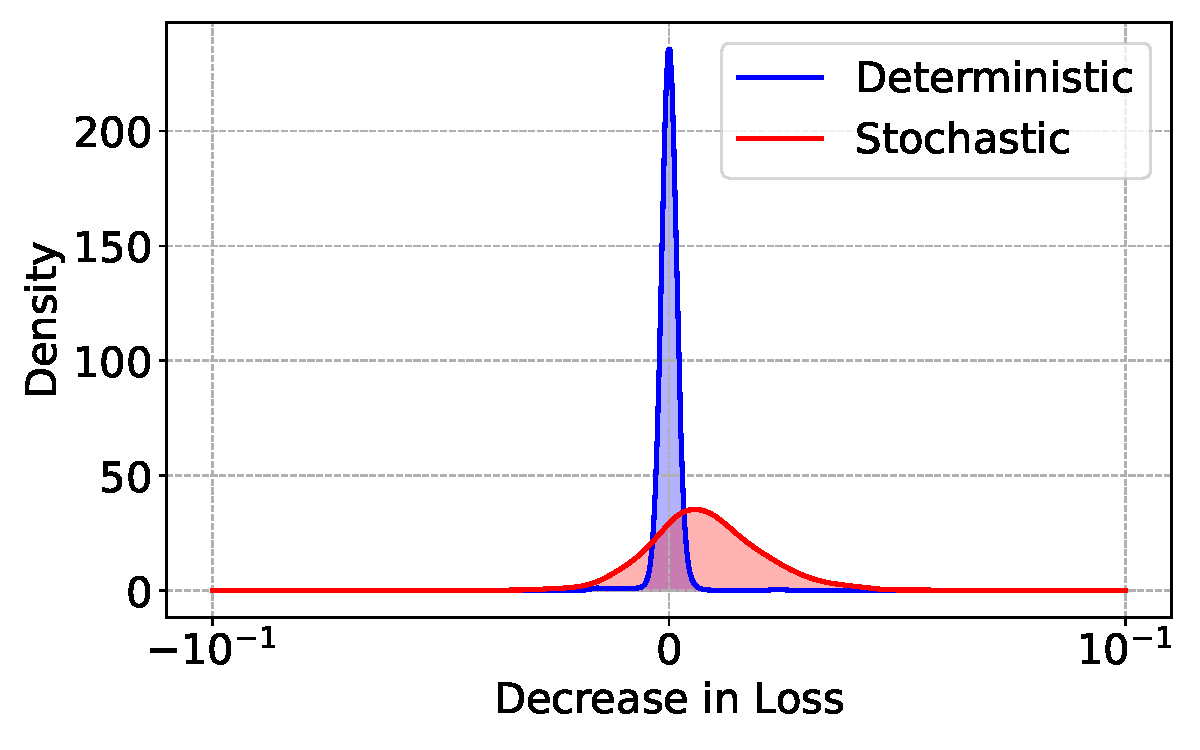
\includegraphics[width=\textwidth]{figures/arxiv/decrease.pdf}
    \end{subfigure}
    \caption{\textbf{Loss Curves and Relative Loss Decrease Distribution.} The left figure reproduces the non-traditional loss curve of $\wsd$ on the synthetic language, showing that the loss remains elevated during the stable phase but sharply declines during the decay phase. The right figure displays the distribution of the relative loss difference from the two different distributions comparing the stable phase and the decay phase. We can observe that the loss decrease over the stochastic distribution is much larger than the decrease in the deterministic distribution. }
    \label{fig:toy}
\end{figure}
\textbf{Empirical Verification.} 
We empirically verify that the loss curve of $\wsd$ can be reproduced in our synthetic setting. The dataset used contains two types of cities: (1) a deterministic type with name distribution's entropy less than 0.2, and (2) a stochastic type with name distribution's entropy greater than 1. Each type contains 1.8k cities and there are 10 possible names. We first train a toy model on this synthetic data and successfully replicate the non-traditional loss curve of $\wsd$ (\Cref{fig:toy},left).




Next, we convert the data into a synthetic language in the format "The resident of [CITY]: [NAME]" and fine-tune a GPT-2 model, pretrained on OpenWebText, using this synthetic data. We experiment with two different learning rate schedules: a constant schedule (stable) and a decaying schedule (decay).
We then calculate the difference in loss between the two models' predictions for the first token of "[NAME]". A significant Spearman correlation of 0.388 (\Cref{fig:toy},right) is observed between the loss difference and the ground truth entropy per city. This correlation indicates that the loss decrease is greater during the decay phase for more stochastic populations. Furthermore, although the decay phase achieves a lower overall loss, the mean loss for the deterministic sub-population is slightly higher than in the stable run, suggesting that the stable run better learns the deterministic sub-population.

